As mentioned in section~\ref{sec:data_extraction} it is both possible and very
easy to access data directly from the database using either direct SQL
statements or programming. This is practical for the cases where it is
desired to perform data treatment on the data or to produce high quality
graphs. However, typically it is sufficient to simply look at the data
and possibly perform light data treatment. For this kind of data analysis it
would be highly impractical to write small custom pieces of software for each
kind of data that the users wish to look at. For this reason we have developed
a framework for visualization of the stored data that allows quick and easy
access to all data. The framework includes support for basic data treatment as
well as the option to plot several data sets at the same time for easy
comparison of results and to export the data to local files. An example of the
web interface used for plotting is shown in Figure~\ref{fig:webinterface}.
\begin{figure}
 \begin{center}
 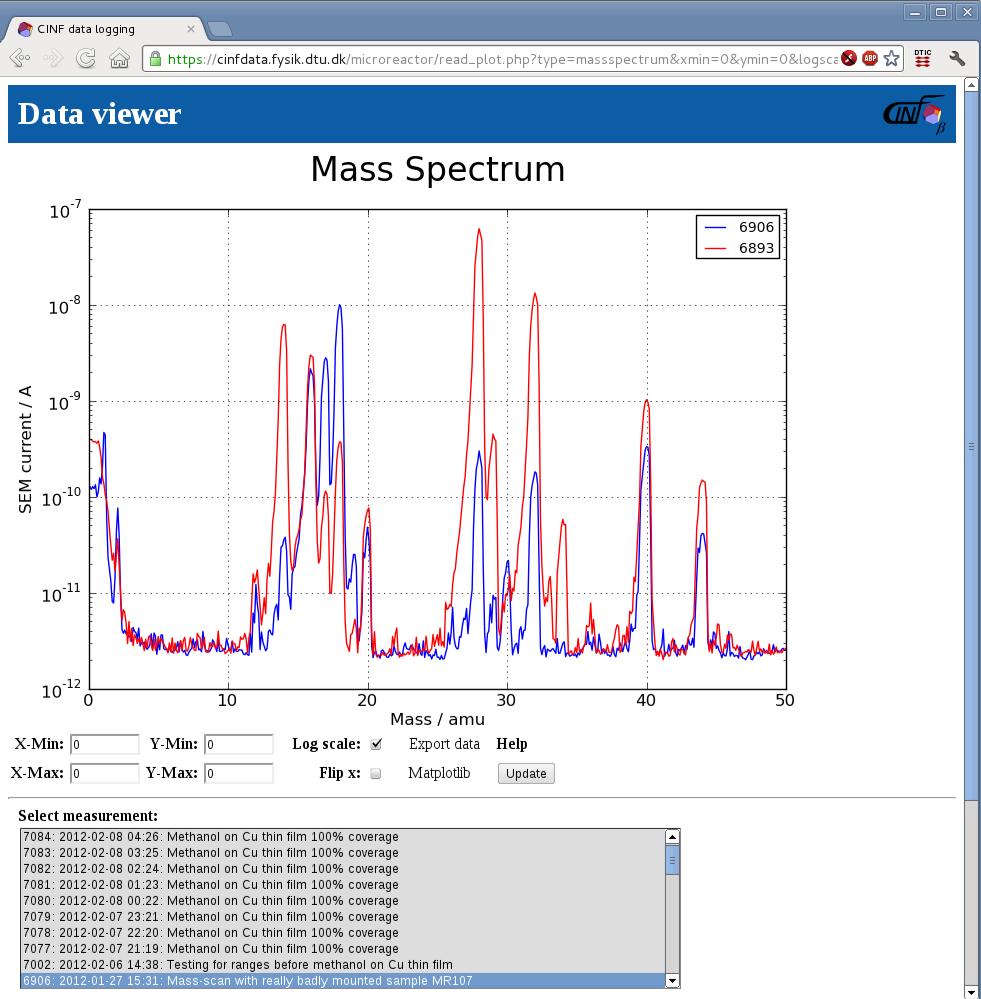
\includegraphics[width=10cm]{mass_spectra_comparison.png}
 \caption{Demonstration of the visualization interface. Data (here mass
   spectrometer data) can be plotted and compared in a web browser allowing
   easy comparison between data. \label{fig:webinterface}
 } 
 \end{center}
\end{figure}

The goal for the visualization module has not been to provide high quality
plots since this is a large task that is best solved with either dedicated
software suites or custom scripts. Instead, the quality of the plots was
targeted such that it is sufficient for different kinds of everyday use
including presentations at informal group meetings, as starting point for
discussion of data, quick data comparison etc. To realize this form of
visualization a frontend/backend topology has been implemented. The code that
handles user input is retrieved in HTML and PHP thus allowing user input to be
acquired from a web browser. The backend consists of an open source plotting
library, interface code to feed data into the plotting code and plot
preferences specific to each experimental setup. The backend is mainly written
in Python and the configuration read from a XML file unique to each setup. The
preferences file contain a settings section for each different kind of plot.
Below is shown an example of a continuously logged pressure:

\begin{verbatim} 
<!-- PRESSURE --> 
<graph type='pressure'>
  <query>SELECT unix_timestamp(time), pressure FROM pressure_SETUP
  where  time between " {from}" and "{to}" order by time</query>
  <ylabel>Pressure / Torr</ylabel>
  <title>Pressure in {setup}</title>
  <default_yscale>log</default_yscale>
  <default_xscale>dat</default_xscale>
</graph>
\end{verbatim}

The system is flexible towards choice of plotting library which is a great
advantage since different plotting libraries are optimal for different tasks.
At the moment the default plots are produced by JavaScript based
dygraphs\cite{dygraphs} allowing real-time manipulation of the data using a
mouse through an ordinary web browser. As a testimony to the flexibility of the
setup matplotlib\cite{matplotlib} is also implemented and can also be used for
visualizing data if the user(s) wishes. Matplotlib produces prettier graphs but at the expense of not allowing dynamic mouse manipulation. JpGraph\cite{jpgraph} has previously
been implemented as plotting library without significant changes to the backend
code demonstrating the large flexibility of system.
